\documentclass{thesis-ekf}             % egyoldalas nyomtatáshoz, elektronikus verzióhoz (fekete linkekkel)
%\documentclass[twoside]{thesis-ekf}    % kétoldalas nyomtatáshoz
%\documentclass[colorlinks]{thesis-ekf} % elektronikus verzióhoz (színes linkekkel)
\usepackage[T1]{fontenc}
\PassOptionsToPackage{defaults=hu-min}{magyar.ldf}
\usepackage[magyar]{babel}
\usepackage[utf8]{inputenc}
\usepackage{listingsutf8,xcolor,caption,graphicx,amsmath,amssymb,amsthm, url, hulipsum}
\footnotestyle{rule=fourth}

\graphicspath{{./kepek/}}

\newtheorem{tetel}{Tétel}[chapter]
\newtheorem{lemma}[tetel]{Lemma}
\theoremstyle{definition}
\newtheorem{definicio}[tetel]{Definíció}
\newtheorem{feladat}[tetel]{Feladat}
\theoremstyle{remark}
\newtheorem{megjegyzes}[tetel]{Megjegyzés}
\newtheorem*{megoldas}{Megoldás}

\begin{document}
\logo{
\includegraphics[width=8cm]{eke-logo.pdf}}
\institute{Matematikai és Informatikai Intézet}
\title{Mobil alkalmazás fejlesztés\\Android platformon}
\author{Balajti-Tóth Kristóf\\Programtervező Informatikus Bsc}
\supervisor{Tajti Tibor\\Egyetemi adjunktus}
\city{Eger}
\date{2019}
\maketitle
\tableofcontents

\chapter*{Bevezetés}
\markboth{Bevezetés}{Bevezetés}
Az szoftver fejlesztés egy nagyon komplex folyamat és rengeteg részletre oda kell figyleni. Az elkészült programnak hatékonynak, hibamentesnek és gyorsnak kell lennie. Természetesen, mindezt határidőn belül kell teljesíteni. Sajnos a biztonság nem egy első számú szempont egy megrendelő szemében,csak akkor ha már valami baj történt. Inkább a gyorsaságon és a folyamatok automatizálásán van a hangsúly, ezért nem  meglepő, hogy a fejlesztés életciklusának tervezési szakaszában kevés figyelem fordul a szoftver biztonságossá tételére.

A statista.com \cite{statista} kutatása szerint 2020-ra több mint 4.78 billió telefon lesz használatban. Ezzel a cégek is tisztában vannak és tudják, hogy ha még több emberhez szeretnék eljuttatni a szolgáltatásukat, akkor rendelkezniük kell saját mobilos alkalmazással.

A mobilos eszközöket célzó támadások száma hatalmas ütemben nő. Mindez azért lehetséges, mert figyelmen kívül marad a ,,secure coding''-nak nevezett gyakorlat. Egy alkalmazásnak a sebezhetőségét különböző támadási vektoron is ki lehet aknázni. Az elején, bennem egy kérdés merült fel. Honnann tudhatom, hogy egy adott alkalmazás sebezhető-e vagy sem. A leghatékonyabb módszer ha visszafejtjük a fájl forráskódra. Ezt angolul ,,reverse engineering''-nek nevezik. A visszaállított fájlok olvashatósága nem lesz tökéletes, főleg ha obfuszkált \footnote{Az obfuszkáció célja röviden, hogy megnehezítse a visszafejtett kód olvashatóságát.} kóddal állunk szemben, de egy tapasztalt szem így is kitudja szúrni a gyakori hibákat.

A szakdolgozatomban androidos telepítő  fájlok forrás fájlokká való visszaállításáról írok, valamint bemutatom hogyan valósítható meg a kliens-szerver kommunikáció egy REST API és egy androidos alkalmazás segítségével. A project fantázia neve ,,Reverse Droid''.

\chapter{Platformok}\label{platformok}

\section{Szerver}

Olyan szerverre volt szükségem, ami nem túl költséges, de mégis megfelelően testreszabható és gyors tárhelyet biztosít. A választásom a Digitial Ocean felhő szolgáltatására esett. Az oldal felületén lehetőségünk van több, úgynevezett \emph{droplet}-et létrehozni, amik nem mások mint virtuális szerverek. Megadhatjuk milyen disztribúciót szeretnénk telepíteni, jelen esetben én egy Ubuntu Linux 18.10-es verziót telepítettem. A telepítés után a droplet IP címét hozzárendeltem egy előre létrehozott subdomain-hez, ezzel biztosítottam, hogy név alapján is elérhető legyen a szerver.

\begin{figure}[!h]
	\centering
	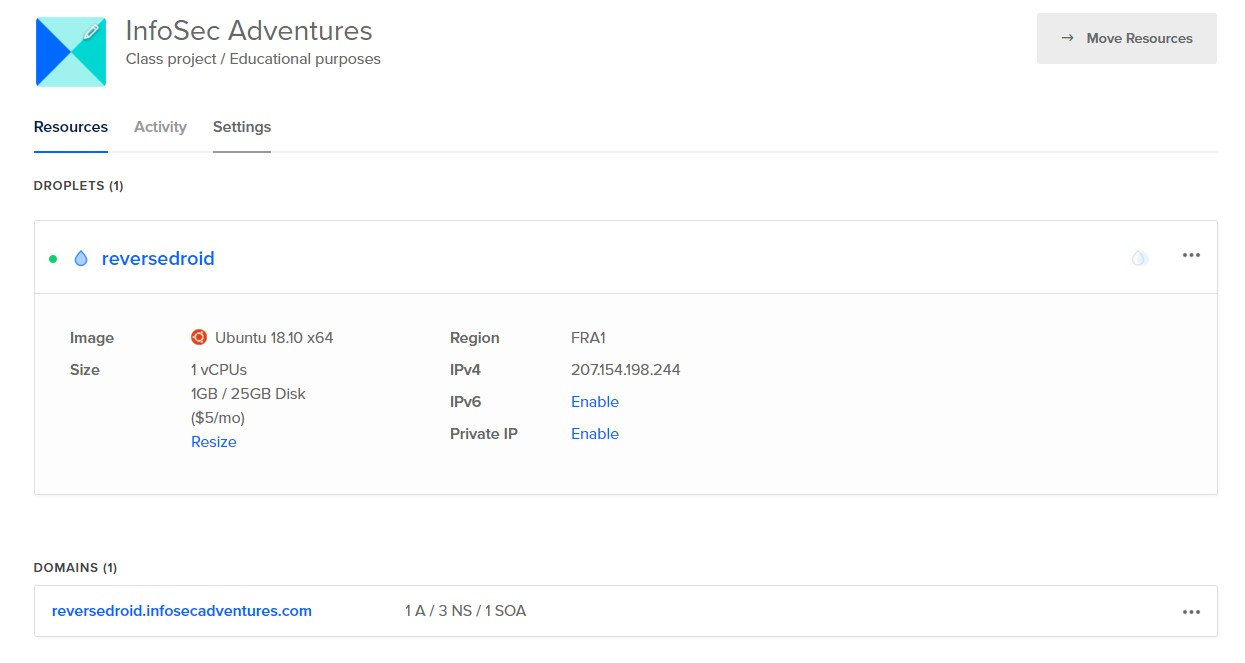
\includegraphics[width=15cm]{kepek/digitalocean}
	\caption{Digital Ocean admin felület.}
	\label{digitalocean}
\end{figure}

\section{Mobil}

A mobilos operációs rendszerek közül az Androidot választottam. Már régebben is sikerül megismerkednem az Android nyújtotta lehetőségekkel és előnyökkel.

\chapter{Felhasznált technológiák}\label{technologiak}

\section{Szerveren használt technológiák}

\section{Androidon használt technológiák}

\begin{thebibliography}{1}
\bibitem{statista} \textsc{ONLINE}: Number of mobile phone users worldwide from 2015 to 2020, \url{https://www.statista.com/statistics/274774/forecast-of-mobile-phone-users-worldwide}
\end{thebibliography}
\end{document}